\documentclass[12pt,a4paper,oneside]{report}

% Formatting stuff:
\setlength{\textheight}{22cm}
\setlength{\textwidth}{16cm}
\setlength{\oddsidemargin}{0cm}
\setlength{\evensidemargin}{0cm}
\setlength{\topmargin}{0cm}
\setlength{\parindent}{0cm}
\setlength{\parskip}{0.8ex}

% Packages required
\usepackage{listings}
\usepackage{natbib}
\usepackage{fancyhdr}
\usepackage[english]{babel}
\usepackage[utf8]{inputenc}
\usepackage[normalem]{ulem}
\usepackage{setspace}
\usepackage{url}
\usepackage{graphicx}
\usepackage{float}
\usepackage{titlesec}
\useunder{\uline}{\ul}{}
\def\code#1{\texttt{#1}}
\setcounter{secnumdepth}{4}
\renewcommand\thesection{\arabic{section}}

% Start
\begin{document}

% Title page
\begin{titlepage}
	\centering
	{\scshape\LARGE Needs Assessment Document \par}
	\vspace{1cm}
	{\scshape\Large MAPme Android Application\par}
	\vspace{1.5cm}
	{\LARGE Authors: D.G. Smith, P.S. Sebeikin\par}
	\vspace{2cm}
	{\large \today\par}
\end{titlepage}
\tableofcontents
\pagebreak
% Body
% discusses the problem area that we are dealing with
\section{Problem Statement}
  \begin{spacing}{1.4}
    The current system is a web-based application that runs within a desktop environment and lacks mobile phone support.  According to the client, it has proved to be inefficient and lacks user-friendliness.  Much of the information, such as the GPS coordinates, must be entered manually.  This creates the possibility of error when data is submitted to the web application.

    The project aims to improve on this system and to develop a mobile smartphone application that will improve user-friendliness, efficiency and provide a convenient method in which to upload submissions to the digital library, thereby supporting the various projects that have requested this app.  It will provide various features that simplify the existing process.  This app will be deployed alongside the web application.  The existing web-based system will remain functional.

    The application will be developed for the Android operating system and will not support any other operating system available. The primary motivation for this is the project team's accessibility to the Android Studio Integrated Development Environment (IDE).  To further motivate this decision, Samsung Android-based devices are the most popular mobile smartphones in South Africa \footnote{http://www.fin24.com/Tech/Gadgets/samsung-dominates-sa-smartphone-tablet-sales-20160329}.
  \end{spacing}

% Describes the existing system that is in place
\section{Existing Implementation}
  \begin{spacing}{1.4}
    The existing web application is on the Animal Demography Unit Virtual (ADU) Museum website\footnote{http://vmus.adu.org.za/}.  From here the user can select which project they wish to submit to. It includes projects such as FishMAP and OrchidMAP.  An ADU account can be created by clicking on ``Registration".  The user's email address has to be entered to check if an account exists
    already.  If not, a screen pops up allowing the creation of an account.  Required information includes an email address, surname, first name and password.  Additional information can be entered including telephone numbers and a postal address.

    A new submission can be created by selecting the ``Data Upload" link on the left hand column of the page. The page has various text fields that the user can fill out with mandatory fields marked by a ``*".  GPS coordinates are entered manually or by means of navigating a Google Maps widget.  The page appears to be cumbersome in its design, with text being small and difficult to read which does not complement the application target market. Once the user has entered the required information, the page allows the user to submit up to three records, specifying which project they belong to.  Furthermore, the page has text fields that are often repeated.  As such, it is difficult for the user to select the correct project and a mistake can easily be made.  This is particularly apparent if the site is visited on a mobile device.  Ultimately the site does not make use of good human computer interaction (HCI) principles. The following image shows the original implementation:
    \begin{figure}[H]
			\centering
      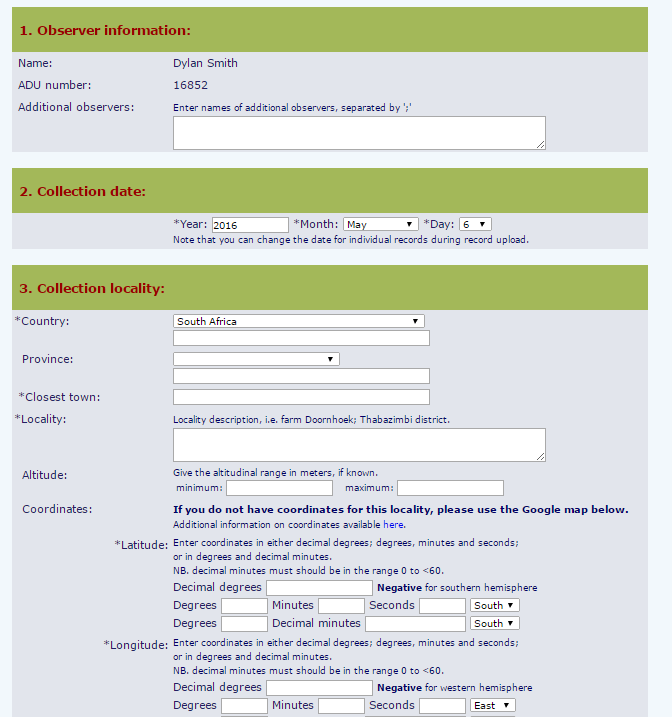
\includegraphics[width=12cm]{existing}
      \caption{Existing web application}
    \end{figure}
  \end{spacing}

  The development of a mobile application will aim to correct the issues of the current implementation.  It will provide
  convenience and ease of use when submitting images to the repository.  The new design will conform to HCI principles to provide this.  Additional features will be added to provide a more rich user experience. Ultimately the design will be user-focused.
% Describes the user base of the app
\section{Target Market}
  \begin{spacing}{1.4}
    The mobile application is aimed at an elderly user group; mostly retirees.  Therefore, the design must be user-friendly, intuitive and as simple as possible to use.  The GUI design will be minimalistic in nature and avoid complex design flows. Various HCI concepts will be considered in the prototype and in the final product to ensure that it complies with the target market of the app.
  \end{spacing}

% Details the user requirements
\section{User Requirements}
\subsection{Mandatory}
    \begin{itemize}
      \item A smooth, simple and intuitive graphical user interface (GUI).
      \item A registration screen that must require the user's email, password and ADU number.
      \item The app must interface with the phone camera.
      \item A photo module that ensures photo quality and consistency (e.g. focus, precision, distance, calibration).
      \item Use of Global Positioning System (GPS) coordinates:
        \begin{itemize}
          \item Interfaced with phone GPS location service
          \item Entered manually by user
          \item Google Maps widget
        \end{itemize}
      \item Photographs should be uploaded immediately or later.  This alludes to the probability of a mobile phone based temporary. data storage structure that holds recorded data until such a time as its upload to the ADU server is initiated.
      \item In the case of animal captures, sound files should be recorded and uploaded (app should interface with the device's voice recorder).
      \item User should be able to enter a locality description.
      \item Must record the date of the submission using the device's set date and time.
			\item The application should enforce mandatory entries and allow optional entries.
      \item The user should optionally be able to specify the species.
      \item The user should optionally be able to enter any other relevant observations.
      \item The user must be able to submit to a particular project (e.g. OrchidMAP, FrogMAP, MammalMAP etc.).
      \item Include a history of user record submissions, to be stored locally on the device that is being used for the submissions.
    \end{itemize}
\subsection{Secondary}
    \begin{itemize}
      \item The user can voice record notes on the submission.  This can be used to detail the surroundings of a plant or specimen.
      \item Option to specify whether the flower or fruit is visible in the submitted image (this will depend on what project it belongs to).
    \end{itemize}
\section{Challenges}
  \begin{spacing}{1.4}
    The obvious challenge is cross-platform compatibility. This means that the app's development is limited to the Android OS.

    Another challenge is the ability to ensure that the photograph submitted by the user is of sufficient quality. This will require a sophisticated development technique that could prove to be a challenge.

    Ensuring the accuracy of GPS locations will also require some thought. The location must be possible and not a contrived location.

    Hardware challenges could be significant. Since Android runs on a wide variety of hardware devices, system resources would vary. This needs to be taken into account during the development process to ensure that the app runs smoothly and is stable on all devices.

    A significant testing framework will need to be developed, such as unit testing (junit in Java) to ensure functionality works as expected. This will also provide a form of quality assurance.

		The project has had little experience developing mobile applications.  The significance of this challenge is directly linked to how quickly the team is able to grasp the Android Studio IDE and its interface with the ADU database which the project team currently has no knowledge of.
  \end{spacing}
\section{Possible Future Enhancements}
  \begin{spacing}{1.4}
    A major enhancement would be to develop the app for other operating systems and not just Android devices. This would greatly expand the app's user base.

    In terms of ensuring image quality, some form of image processing technique can be used to automatically detect plant attributes. This can also be used to ensure image quality.
  \end{spacing}
\section{Summary}
  The goal is to develop an easy-to-use, smooth and well-performing app that is effective and efficient to aid the Virtual Museum Project.
  It will correct the problems that reside in the existing implementation and introduce ease and convenience.
\end{document}
